\documentclass{article}
\usepackage{../report}
\graphicspath{ {./imgs} }
\title{Lab 4 Report}

\begin{document}
\maketitle
\section{Introduction}
In this lab we are only analyzing one circuit. This is
the circuit shown in Figure \ref{maincircuit} and it features
the 2N2700 MOSFET device known as a 2N2700. In this lab we 
aren't using that device as it is intended to be used, but 
rather we are going to be putting the device under unusual 
circumstances. This ended up resulting in some irregular 
patterns in our measurements as you'll see later in the lab
report.

A MOSFET device is one that allow us to effectively "flip" a 
switch electronically by supplying a voltage into 
the device which determines if current should or shouldn't 
flow through the other portion of the device.

\begin{figure}[h!]
  \begin{center}
  \begin{circuitikz}[american]
    \ctikzset{tripoles/mos style/arrows}
    \def\killdepth#1{{\raisebox{0pt}[\height][0pt]{#1}}}
    \draw (0,0) node[ground]{} to
    [voltage source, v^=v$_{gs}$, invert] ++(0,2) to (1,2);
    \draw (2,2) node[nmos](Q1){\killdepth{2N2700}};
    \draw (2,1.25) to (2,0) node[ground]{};
    \draw (2, 2.75) -- (2,3) -- (4,3) to [voltage source, v^=v$_{ds}$] (4,0) node[ground]{};
  \end{circuitikz}
  \caption{Circuit Featuring an NMOS IV Component}
  \label{maincircuit}
  \end{center}
\end{figure}

\section{Sweeping the V$_{gs}$}
For the first portion of the lab we set up the circuit as 
shown in Figure \ref{maincircuit}, and we kept the value of V$_{ds}$
constant at 5 V while sweeping the value of V$_{gs}$. By doing
this we are analyzing at what value V$_{gs}$ does the MOSFET "turn
on" and allow current to flow through the other portion of the 
device. As you can see from Figure \ref{results1}, the current
flowing through the device just started to flow at about V$_{gs}=2.2$ V
and made a significant jump at v$_{gs}=2.3$ V. Essentially, when the
voltage reached 2.3 volts you could consider the transistor as "turned
on" and significant current was then flowing through the circuit.

These findings match our simulation from Multisim as shown in Figure 
\ref{simcurrentstarts}.
\begin{figure}[!htb]
  \begin{center}
    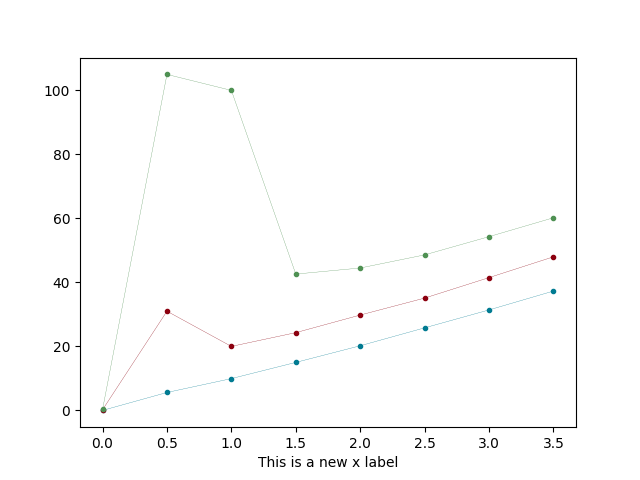
\includegraphics[width=0.7\textwidth]{imgs/meas/sweepvgs}
  \end{center}
  \caption{Results from Sweeping the V$_{gs}$ Value}
  \label{results1}
\end{figure}
\begin{figure}[!htb]
  \begin{center}
    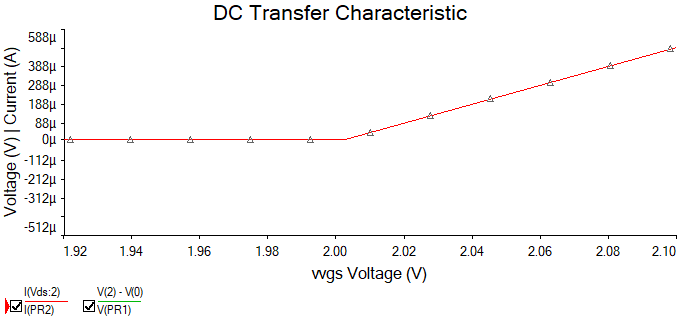
\includegraphics[width=0.7\textwidth]{imgs/sim/Id vs Vgs current starts}
  \caption{Simulation of Current Starting to Flow}
  \label{simcurrentstarts}
  \end{center}

\end{figure}

\section{Sweeping the V$_{ds}$}
In this second portion of the lab we were tasked with 
sweeping the value of the V$_{ds}$ voltage which 
is where the current that we are measuring is coming from.
The point of this is to see how different voltage values of 
V$_{gs}$ will affect the current output of the transistor.
As you can see in Figure \ref{multiplecurrents}, the value of 
V$_{gs}$ will change the current throughput of the transistor 
for the different ranges of V$_{ds}$. Our measurements showed
a similar trend, though the results were affected by some 
unknown factor at the lower voltages of V$_{ds}$. Because
of this unknown factor we found that there was an 
apparent bump in our graphs, and we couldn't find a way
to prevent that. Regardless, we were able to determine
that there was a consistent difference in the current 
throughput as the V$_{gs}$ voltage changed. The higher 
the V$_{gs}$ voltage, the higher the I$_D$ output.

\begin{figure}[!htb]
  \begin{center}
    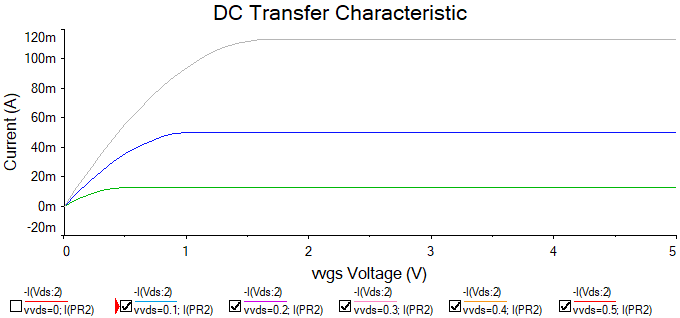
\includegraphics[width=0.7\textwidth]{imgs/sim/Id vs Vds}
  \caption{Currents Simulated for Various V$_{gs}$ Values}
  \label{multiplecurrents}
  \end{center}
\end{figure}

Our measurements from this portion of the lab can be seen in 
Figure \ref{results2}.

\begin{figure}[!htb]
  \begin{center}
  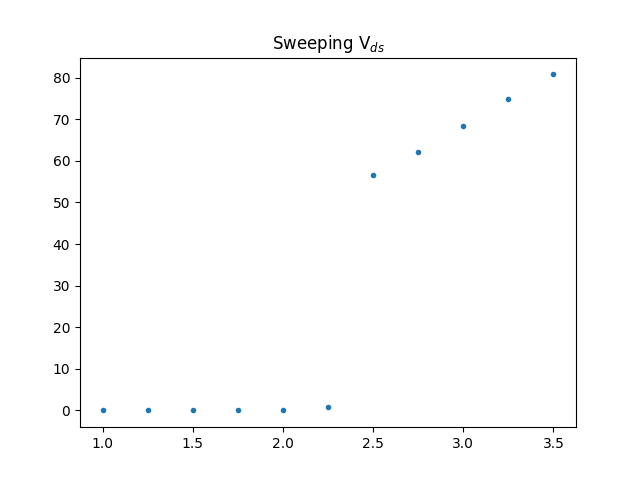
\includegraphics[width=0.7\textwidth]{imgs/meas/sweepvds}
  \caption{Results from Measurements when Sweeping V$_{ds}$}
  \label{results2}
  \end{center}
\end{figure}
  
\section{Conclusion}
In this lab I was able to learn a little bit more about 
the function of MOSFET transistors. It's been interesting
learning in this class about the details behind
semiconductors and how they function in more detail. It's 
apparent why these are used so much in digital circuits 
because they seem to show such a binary response to stimulus,
though I'm sure there are plenty of uses in analog circuits 
as well. I'd be interested in learning more about the analog 
applications of MOSFET and other transistors. It was interesting
learning in this lab about the different behavior of the 
2N2700 transistor when different voltage levels were
applied.

\end{document}